\chapter{Introduction}
Dans ce rapport nous allons utiliser un Arduino Uno ainsi que toute une série de modules compris dans un coffret. Arduino est une plateforme de développement open source via des cartes de développement. Puisque le projet est open source, les schemas des cartes est disponnible gratuitement ainsi que la suite logicielle Arduino que nous avons utilisé dans ces manipulations.
L'Arduino que nous utilisons est l'Arduino Uno qui possède 14 entrés/sortie numérique dont 6 sont compatibles PWM et 6 entrées/sorties analogiques. Il possède également une prise USB pour injecter notre code ou pour l'alimenter et une prise d'alimentation jack. Efin, un bouton reset est présent pour `rebooter' l'Arduino.
\begin{figure}[h]
	\centering
	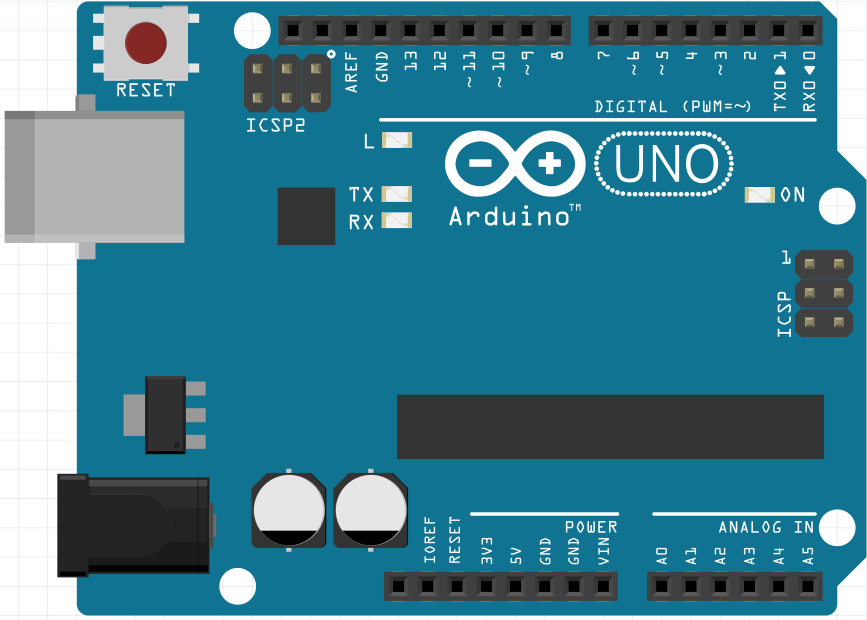
\includegraphics[height=3cm]{img/arduino.png}
	\caption{\label{ArduinoBoard}Arduino Board}
\end{figure}
Pour la programation de l'Arduino nous utillisons la suite officielle d'Arduino disponible gratuitement. Pour les schematiques nous avons utilisé Fritzing, également fournis gratuitement par la fondation Arduino.
\begin{figure}[h]
	\centering
	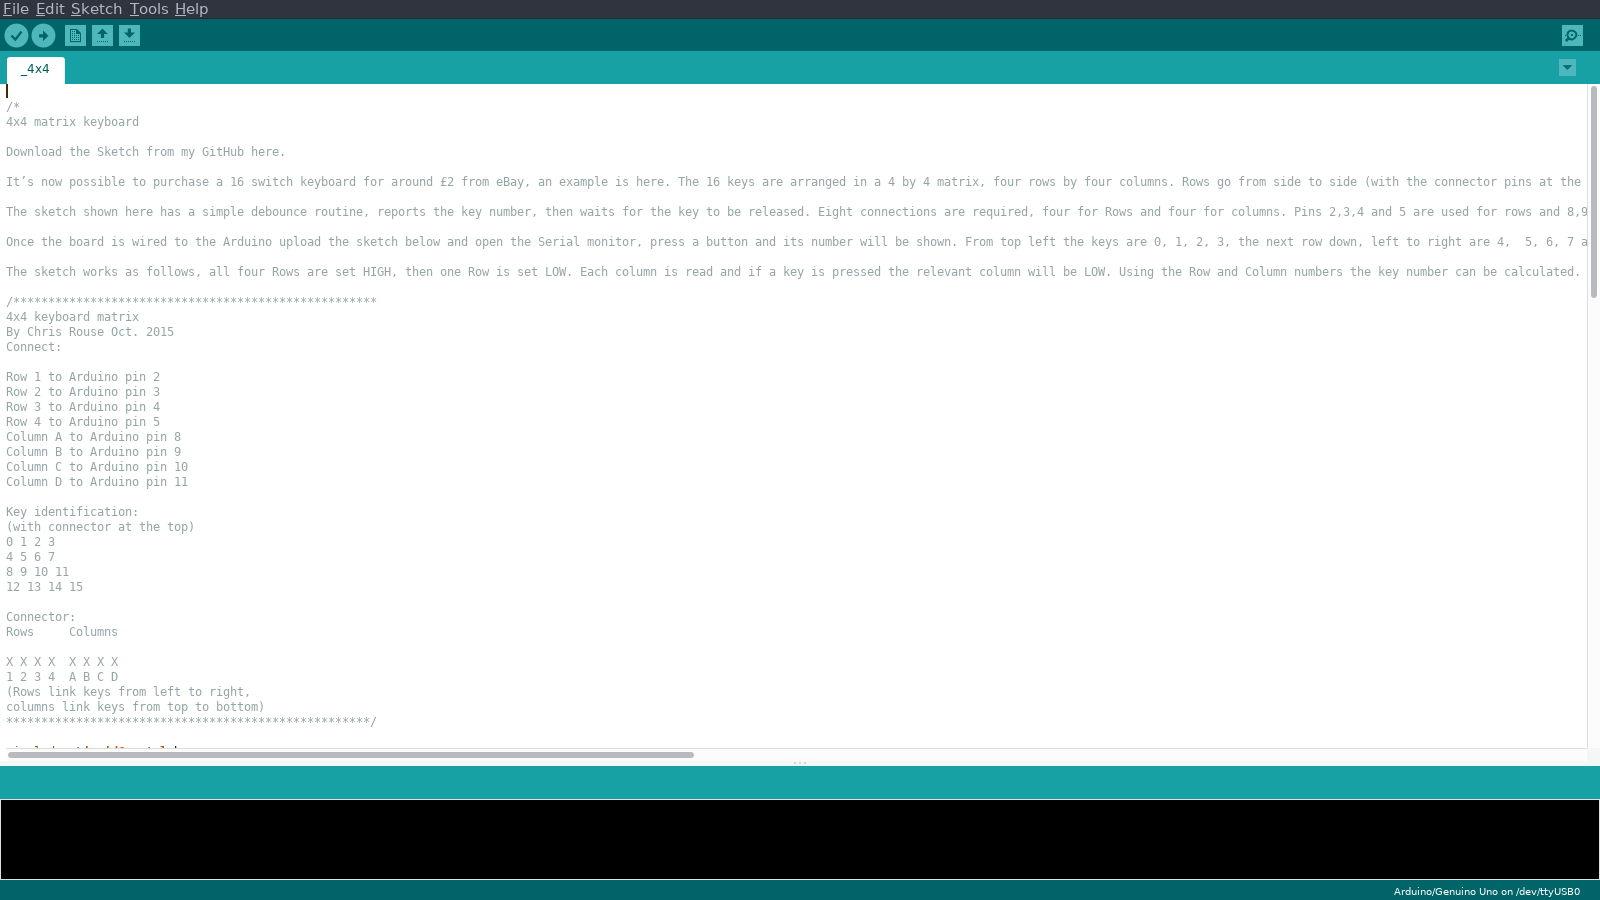
\includegraphics[height=6cm]{img/suite.png}
	\caption{\label{SuiteArduino}Suite Arduino}
\end{figure}
\begin{figure}[h]
	\centering
	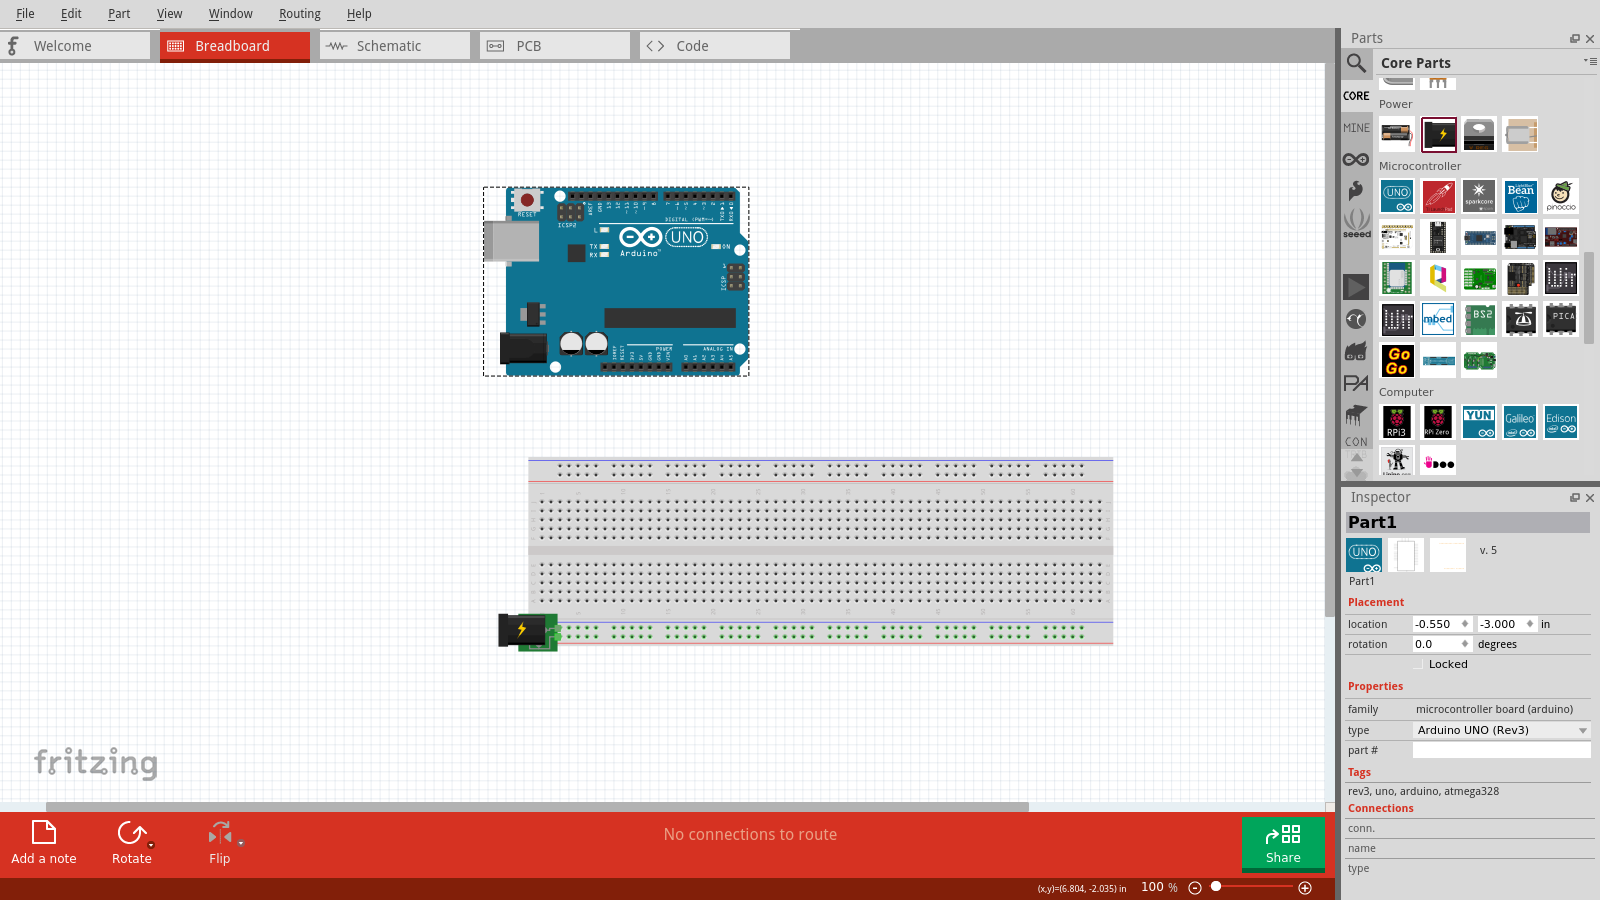
\includegraphics[height=6cm]{img/fritzing.png}
	\caption{\label{Fritzing}Fritzing}
\end{figure}